\section{tasks::blazecorr Class Reference}
\label{classtasks_1_1blazecorr}\index{tasks::blazecorr@{tasks::blazecorr}}
Inheritance diagram for tasks::blazecorr::\begin{figure}[H]
\begin{center}
\leavevmode
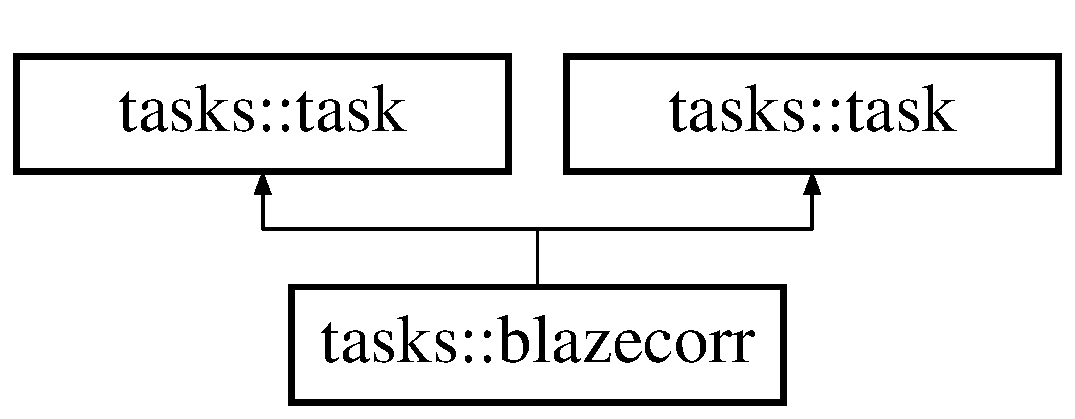
\includegraphics[height=2cm]{classtasks_1_1blazecorr}
\end{center}
\end{figure}
\subsection*{Public Member Functions}
\begin{CompactItemize}
\item 
def \textbf{run}\label{classtasks_1_1blazecorr_cbf816168701d529dfbad7d281989b5e}

\item 
def \textbf{run}\label{classtasks_1_1blazecorr_cbf816168701d529dfbad7d281989b5e}

\end{CompactItemize}
\subsection*{Static Public Attributes}
\begin{CompactItemize}
\item 
string \textbf{name} = '{\bfblazecorr}'\label{classtasks_1_1blazecorr_5d0a45f69faa7facb9aab8624d9b30ef}

\item 
string \textbf{button\-Text} = 'Correct for blazeshape'\label{classtasks_1_1blazecorr_34011eb4e7330133c7f30a957c8b0a5d}

\item 
string \textbf{suffix} = 'blzcorr'\label{classtasks_1_1blazecorr_53d0151385808cb5ac8d06a7ede50030}

\item 
list \textbf{prereq} = ['{\bfextspec}']\label{classtasks_1_1blazecorr_12a5ab82b194d94af517d77350c34feb}

\end{CompactItemize}


\subsection{Detailed Description}


\footnotesize\begin{verbatim}Divide the extracted orders by the blaze shape, producing flattened spectra.
   There is no additional continuum fitting performed. The blaze shape is taken from
   a pre-determined fit to the combined flat frame.
\end{verbatim}
\normalsize
 



The documentation for this class was generated from the following files:\begin{CompactItemize}
\item 
old/PANICtool-1.0/tasks.py\item 
old/tasks.py\end{CompactItemize}
